\documentclass{beamer}
\mode<presentation>
\usepackage{beamerthemesplit}
\usetheme{Pittsburgh}
\usecolortheme{seahorse}
\usepackage[MeX]{polski}
\usepackage[utf8]{inputenc}
\usepackage{verbatim}
\usepackage{graphicx}
\usepackage{pstricks}
\usepackage{pst-plot}
\usepackage{pst-node}
\author{Autor: Stanisław Swianiewicz \linebreak Opiekun naukowy: dr inż. Piotr Marusak}
\title{Metody identyfikacji i dostrajania \\ modeli rozmytych}
\date{2.\ grudnia 2010 r.}
\setbeamertemplate{footline}{\hspace*{.5\textwidth}\insertframenumber/\inserttotalframenumber}

\begin{document}
\frame{
\titlepage
}

\section*{Plan prezentacji}
\frame{
\tableofcontents
}

\section{Modelowanie rozmyte}
\frame{
  \frametitle{Modele rozmyte Takagi-Sugeno-Kanga}
  \begin{itemize}
  \item Obszar zmienności wejść modelu dzielony na zbiory rozmyte
  \item Funkcje przynależności
  \item Reguły wnioskowania
  \item Liniowe modele lokalne
  \end{itemize}
}
\frame{
\frametitle{Modele rozmyte Takagi-Sugeno-Kanga}
Zbiór reguł --- baza wiedzy
\begin{displaymath}
\begin{array}{l}
\mathrm{R}^1:\mbox{ JEŚLI } x_1 \mbox{ jest } X_{11} \mbox{ i } x_2 \mbox{ jest } X_{21} \mbox{ to } y^{11}=f_{11}(x) \\
\mathrm{R}^2:\mbox{ JEŚLI } x_1 \mbox{ jest } X_{11} \mbox{ i } x_2 \mbox{ jest } X_{22} \mbox{ to } y^{12}=f_{12}(x) \\
\mathrm{R}^3:\mbox{ JEŚLI } x_1 \mbox{ jest } X_{12} \mbox{ i } x_2 \mbox{ jest } X_{21} \mbox{ to } y^{21}=f_{21}(x) \\
\mathrm{R}^4:\mbox{ JEŚLI } x_1 \mbox{ jest } X_{12} \mbox{ i } x_2 \mbox{ jest } X_{22} \mbox{ to } y^{22}=f_{22}(x) \\
\end{array}
\end{displaymath}
}
\frame{
\frametitle{Modele rozmyte Takagi-Sugeno-Kanga}
Funkcje przynależności, wnioskowanie rozmyte
  \resizebox{\textwidth}{!}{
      \begin{pspicture}(12,7)
          \rput(0.5,0.5){
          %\psgrid
          \psaxes[labels=none, ticks=none]{->}(3,3)(3,3)(10,6)
          \psaxes[labels=none, ticks=none]{->}(3,2)(3,2)(10,0)
          \psaxes[labels=none, ticks=none]{->}(2,3)(2,3)(0,6)
          \psline{-}(2.8,0.2)(6,0.2)(7,2)
          \psline{-}(6,2)(7,0.2)(10,0.2)
          \psline{-}(0.2,2.8)(0.2,4)(2,5)
          \psline{-}(2,4)(0.2,5)(0.2,6)
          \psline[linewidth=0.01, linestyle=dashed]{-}(6,0)(6,6)
          \psline[linewidth=0.01, linestyle=dashed]{-}(7,0)(7,6)
          \psline[linewidth=0.01, linestyle=dashed]{-}(0,4)(10,4)
          \psline[linewidth=0.01, linestyle=dashed]{-}(0,5)(10,5)
          \Rput[r](10,2.5){$x_1$}
          \Rput[t](2.5,6){$x_2$}
          \Rput[c](2.5,2.5){$0$}
          \Rput[b](2.5,0){$1$}
          \Rput[l](0,2.5){$1$}
          \Rput[b](4.5,0.2){$\mu _{X_{11}}(x)$}
          \Rput[b](8.5,0.2){$\mu _{X_{12}}(x)$}
          \Rput[l](0.2,3.5){$\mu _{X_{21}}(x)$}
          \Rput[l](0.2,5.5){$\mu _{X_{22}}(x)$}
          \Rput[c](4.5,3.5){$f_{11}(x)$}
          \Rput[c](8.5,3.5){$f_{21}(x)$}
          \Rput[c](4.5,5.5){$f_{12}(x)$}
          \Rput[c](8.5,5.5){$f_{22}(x)$}
          }
      \end{pspicture}
  }
}

\section{Rozmyte sieci neuronowe}
\frame{
\frametitle{Struktura rozmytej sieci neuronowej}
\resizebox{\textwidth}{!}{
      \begin{pspicture}(18,8)
          %\psgrid
          \rput[c](3, 4){\rnode{x1}{$x_1$}}
          \rput[c](2, 0){\rnode{x2}{$x_2$}}
          \rput[c](5, 5){\circlenode{m11}{$\mu _{X_{11}}$}}
          \rput[c](5, 3){\circlenode{m12}{$\mu _{X_{12}}$}}
          \rput[c](5, 1){\circlenode{m21}{$\mu _{X_{21}}$}}
          \rput[c](5, -1){\circlenode{m22}{$\mu _{X_{22}}$}}
          \ncline[nodesepA=3pt]{x1}{m11}
          \ncline[nodesepA=3pt]{x1}{m12}
          \ncline[nodesepA=3pt]{x2}{m21}
          \ncline[nodesepA=3pt]{x2}{m22}
          \rput[c](7, 5){\circlenode{w11}{$\prod$}}
          \rput[c](7, 3){\circlenode{w12}{$\prod$}}
          \rput[c](7, 1){\circlenode{w21}{$\prod$}}
          \rput[c](7, -1){\circlenode{w22}{$\prod$}}
          \ncline{m11}{w11}
          \ncline{m11}{w12}
          \ncline{m12}{w21}
          \ncline{m12}{w22}
          \ncline{m21}{w11}
          \ncline{m21}{w21}
          \ncline{m22}{w12}
          \ncline{m22}{w22}
          \rput[c](9, 9){\circlenode{f11}{$f_{11}$}}
          \rput[c](9, 8){\circlenode{f12}{$f_{12}$}}
          \rput[c](9, 7){\circlenode{f21}{$f_{21}$}}
          \rput[c](9, 6){\circlenode{f22}{$f_{22}$}}
          \pnode(7.5, 8.5){x2p}
          \pnode(7.5, 6.5){x1p}
          \ncangle[nodesepA=3pt, angle=90, armB=0]{x1}{x1p}
          \ncangle[nodesepA=3pt, angle=90, armB=0]{x2}{x2p}
          \ncline{x1p}{f11}
          \ncline{x1p}{f12}
          \ncline{x1p}{f21}
          \ncline{x1p}{f22}
          \ncline{x2p}{f11}
          \ncline{x2p}{f12}
          \ncline{x2p}{f21}
          \ncline{x2p}{f22}
          \rput[c](12, 5.5){\circlenode{y11}{$\prod$}}
          \rput[c](12, 4){\circlenode{y12}{$\prod$}}
          \rput[c](12, 2.5){\circlenode{y21}{$\prod$}}
          \rput[c](12, 1){\circlenode{y22}{$\prod$}}
          \rput[c](12, -1){\circlenode{sum}{$\sum$}}
          \ncline{w11}{y11}
          \ncline{w12}{y12}
          \ncline{w21}{y21}
          \ncline{w22}{y22}
          \ncline{f11}{y11}
          \ncline{f12}{y12}
          \ncline{f21}{y21}
          \ncline{f22}{y22}
          \ncline{w11}{sum}
          \ncline{w12}{sum}
          \ncline{w21}{sum}
          \ncline{w22}{sum}
          \rput[c](14, 3.25){\circlenode{wyn1}{$\sum$}}
          \ncline{y11}{wyn1}
          \ncline{y12}{wyn1}
          \ncline{y21}{wyn1}
          \ncline{y22}{wyn1}
          \rput[c](16, 3.25){\circlenode{wyn2}{$/$}}
          \ncline{wyn1}{wyn2}
          \ncline{sum}{wyn2}
          \rput[c](18, 3.25){\rnode{y}{$y$}}
          \ncline[nodesepB=3pt]{->}{wyn2}{y}
\end{pspicture}
    }

}
\frame{
\frametitle{Algorytm uczenia rozmytej sieci neuronowej}
\begin{itemize}
\item Algorytm hybrydowy
\item Dostrajanie parametrów liniowych następników - metoda najmniejszych kwadratów
\item Dostrajanie parametrów poprzedników - uczenie SN
\begin{itemize}
\item Optymalizacja gradientowa - algorytm propagacji wstecznej
\item Optymalizacja bezgradientowa
\end{itemize}
\end{itemize}
}
\frame{
\frametitle{Algorytm uczenia rozmytej sieci neuronowej}
\begin{pspicture}(18,8)
        %\psgrid
        \rput[bl](0,4){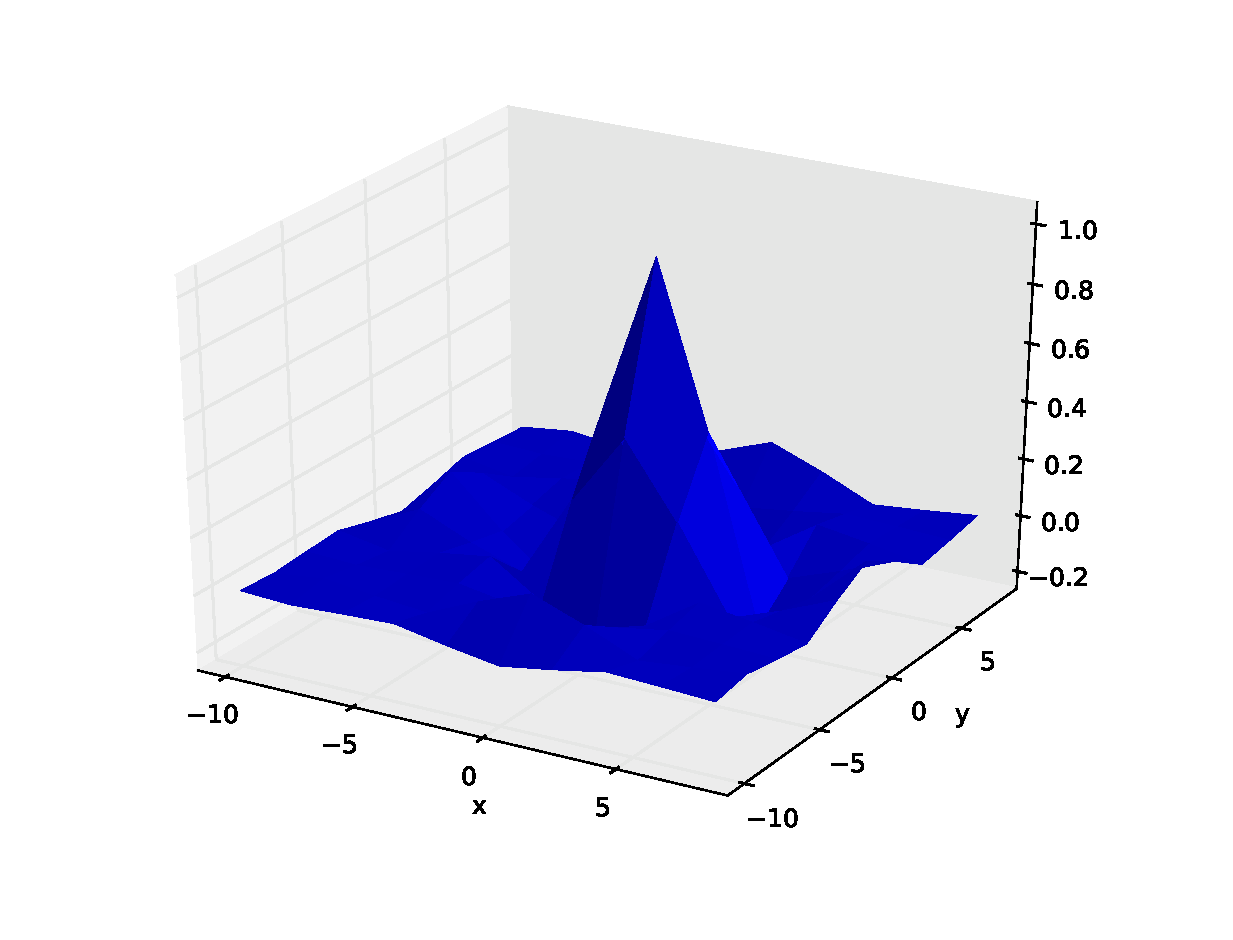
\includegraphics[width = 5cm]{test.eps}}
        \Rput[c](2.5,4){\small dane testowe}
        \pause
        \rput[bl](5,2){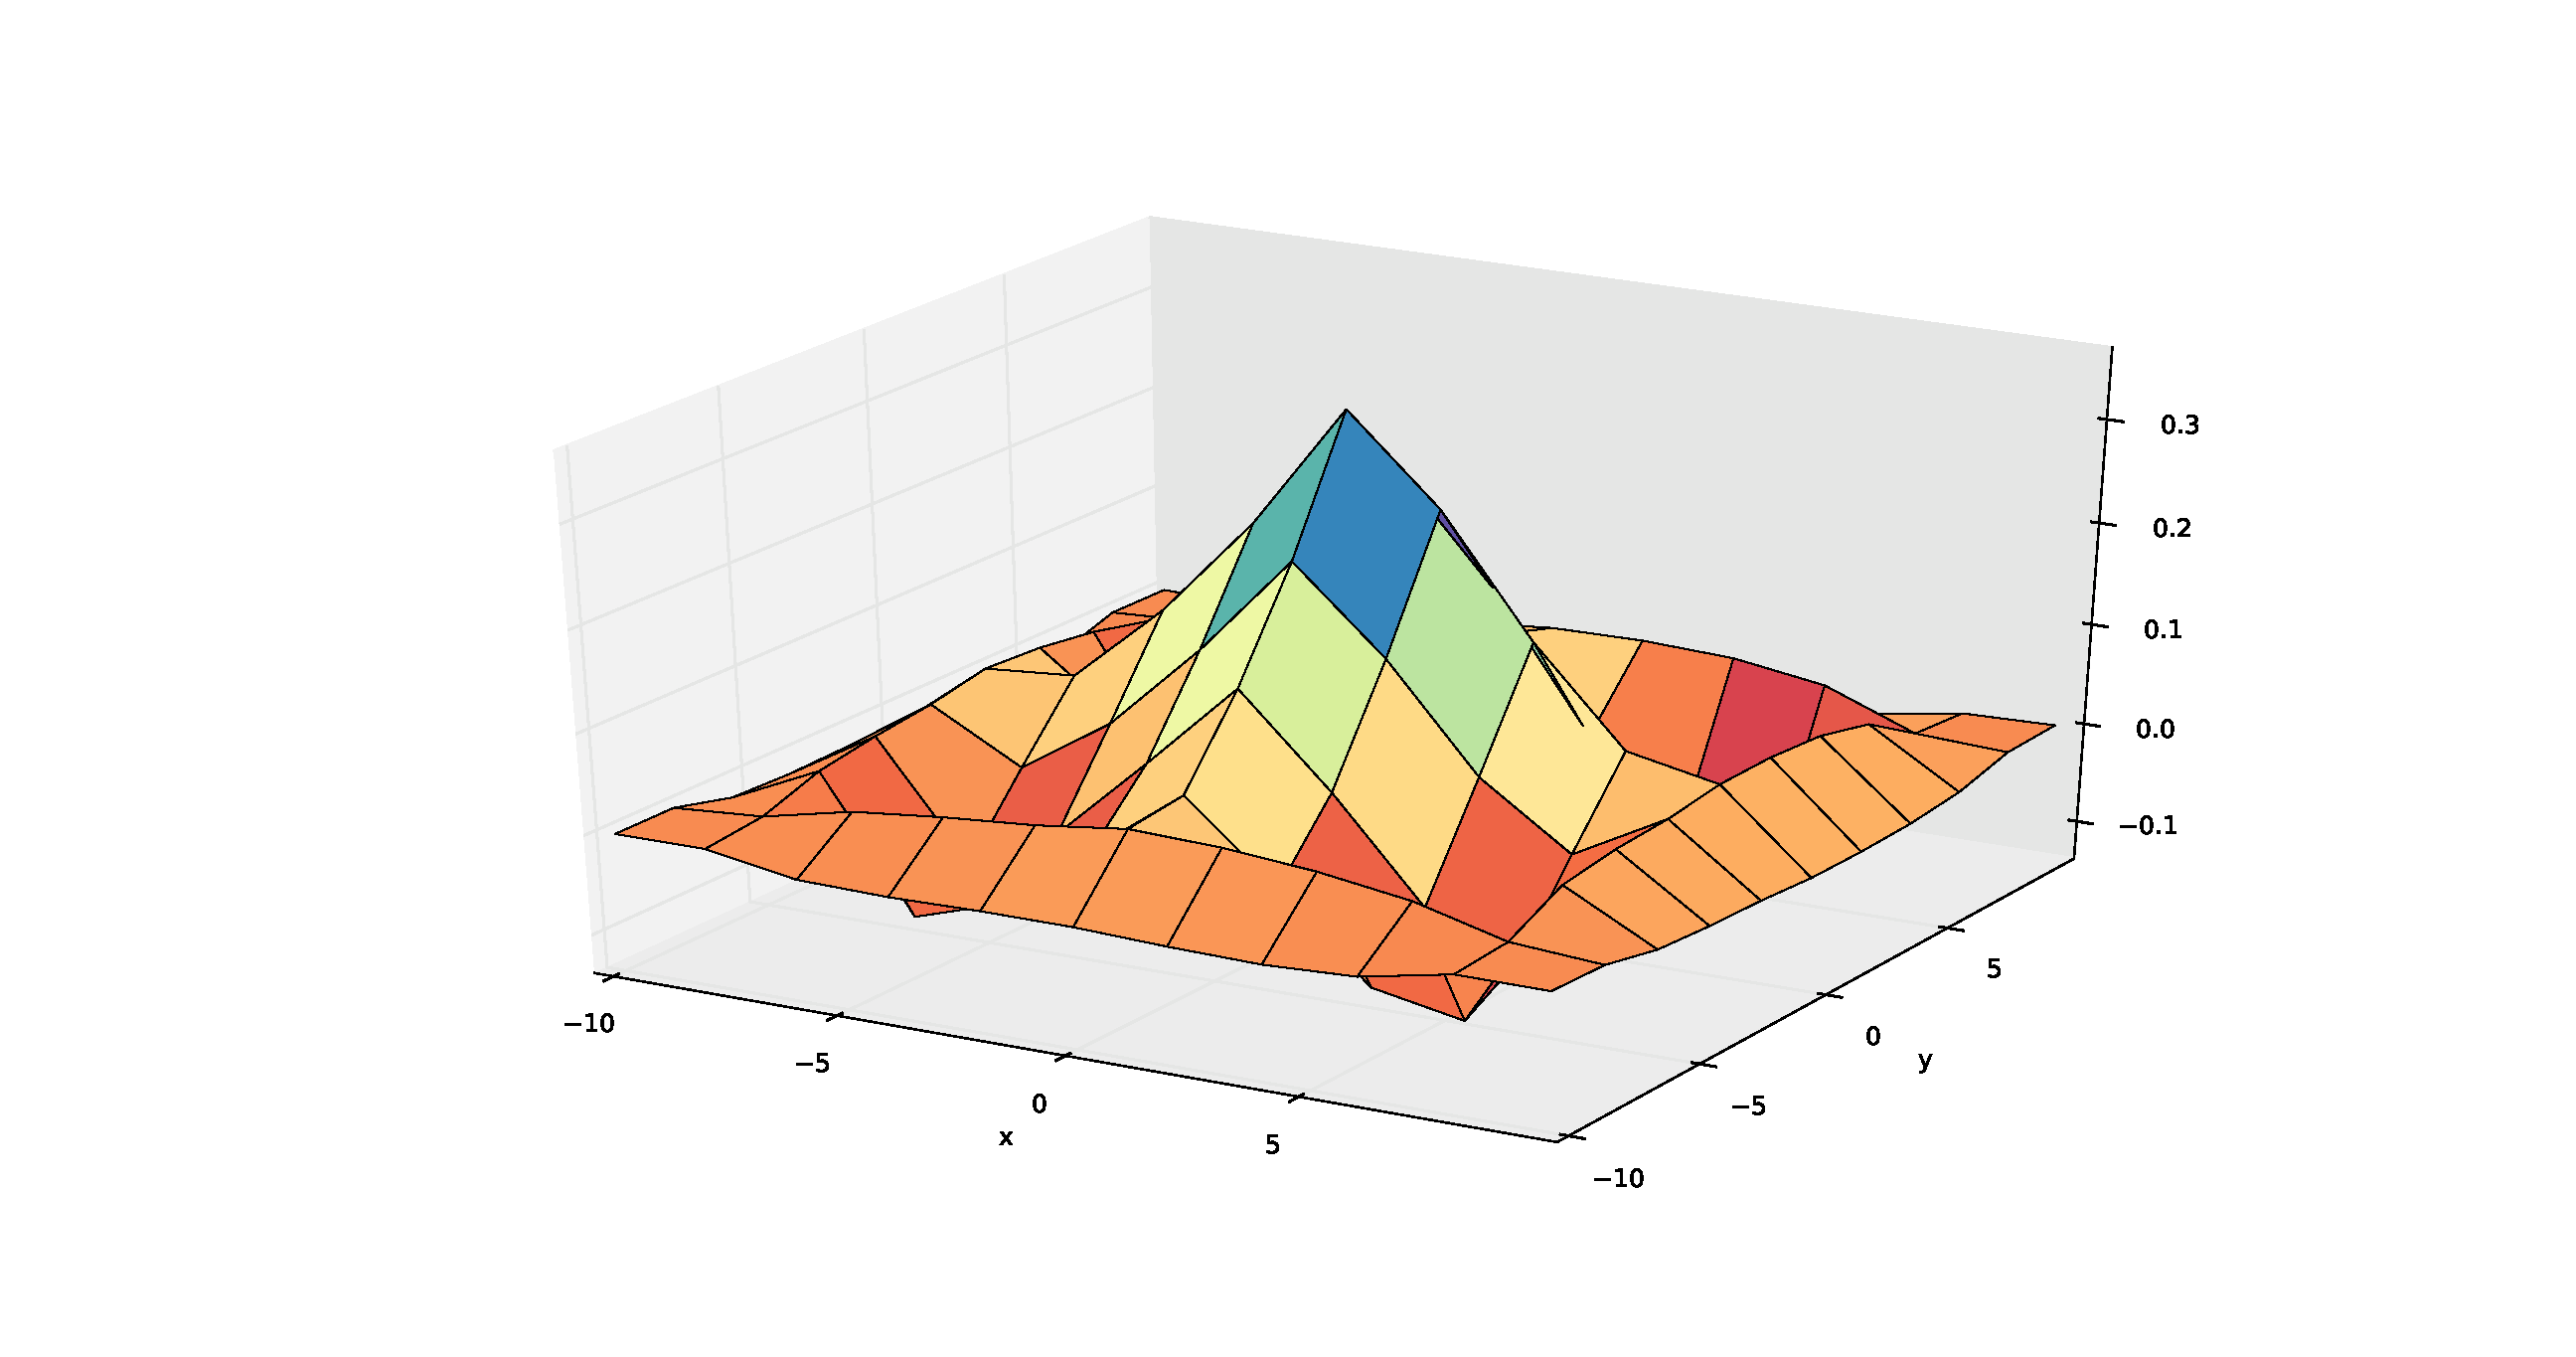
\includegraphics[width = 6cm]{lsq.eps}}
        \Rput[c](8,2){\small następniki dostrojone mnk}
\end{pspicture}
}
\frame{
\frametitle{Algorytm uczenia rozmytej sieci neuronowej}
\begin{pspicture}(18, 8)
        %\psgrid
        \rput[br](11,1.5){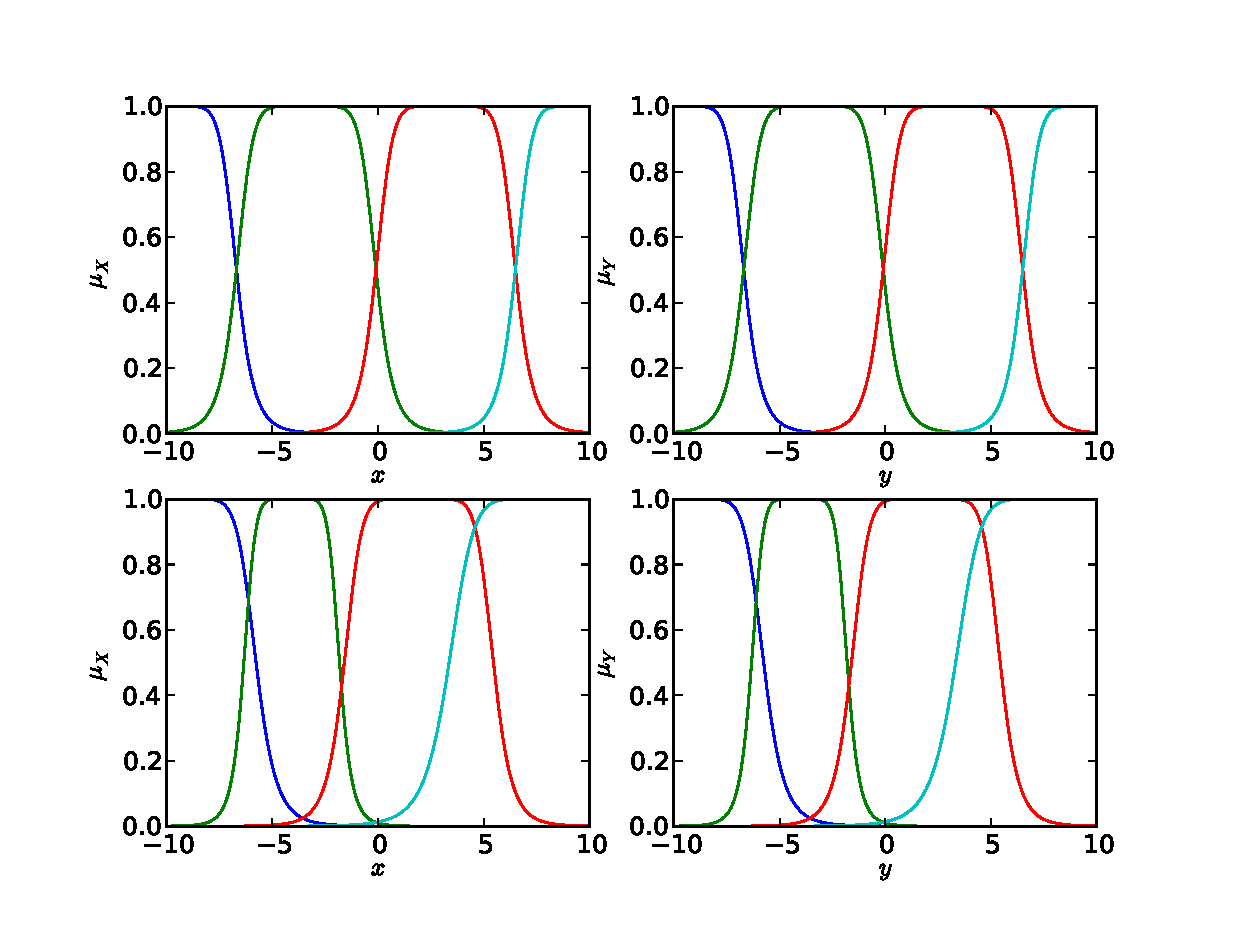
\includegraphics[width = 8cm]{memfunc.eps}}
        \Rput[c](6,7.4){\small funkcje przynależności}
        \Rput[r](3.4,5.9){\small sieć nie uczona}
        \Rput[r](3.4,3.1){\small 50 epok uczenia}
\end{pspicture}
}
\frame{
\frametitle{Algorytm uczenia rozmytej sieci neuronowej}
\begin{pspicture}(18,8)
        %\psgrid
        \rput[bl](0,4){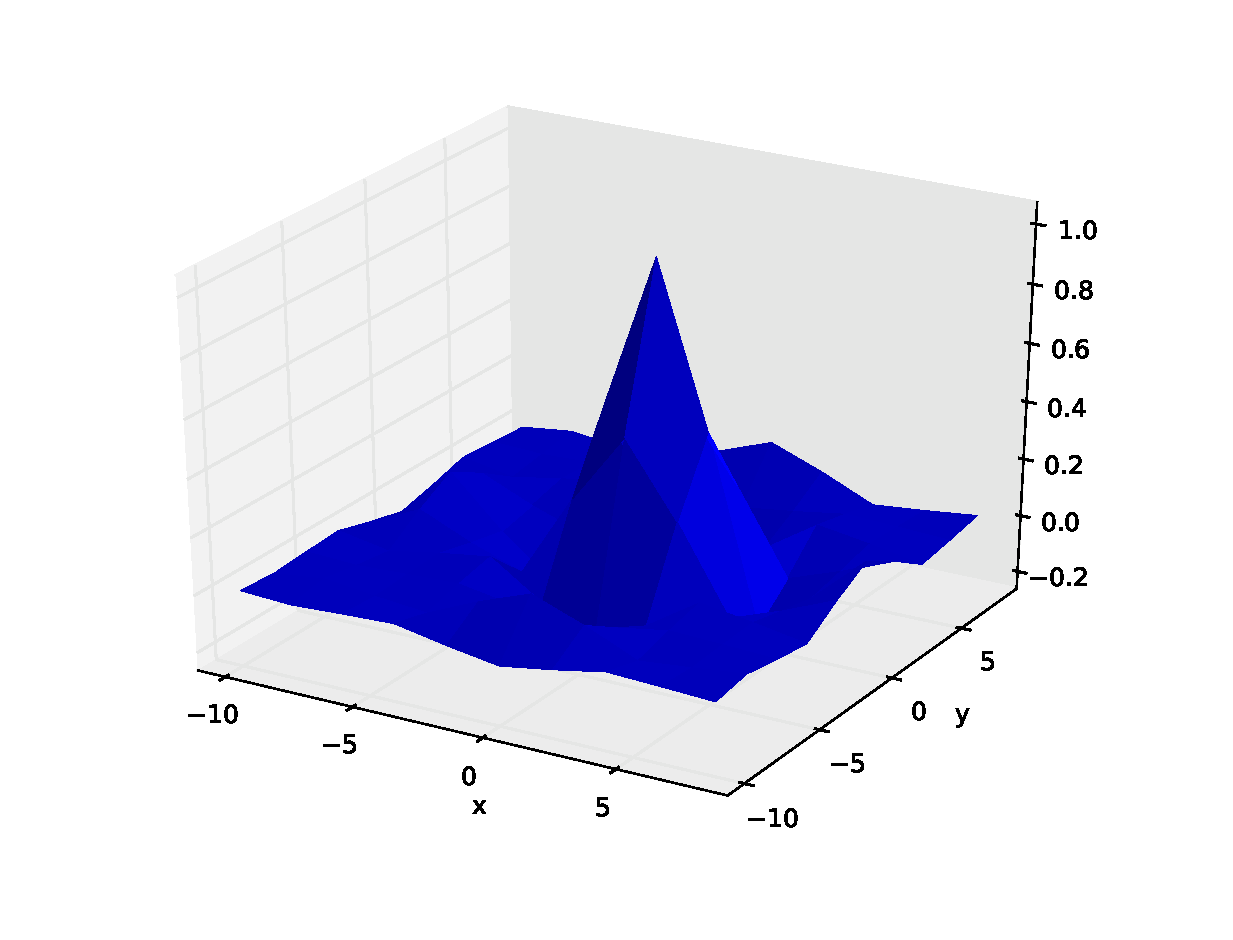
\includegraphics[width = 5cm]{test.eps}}
        \Rput[c](2.5,4){\small dane testowe}
        \rput[bl](5,2){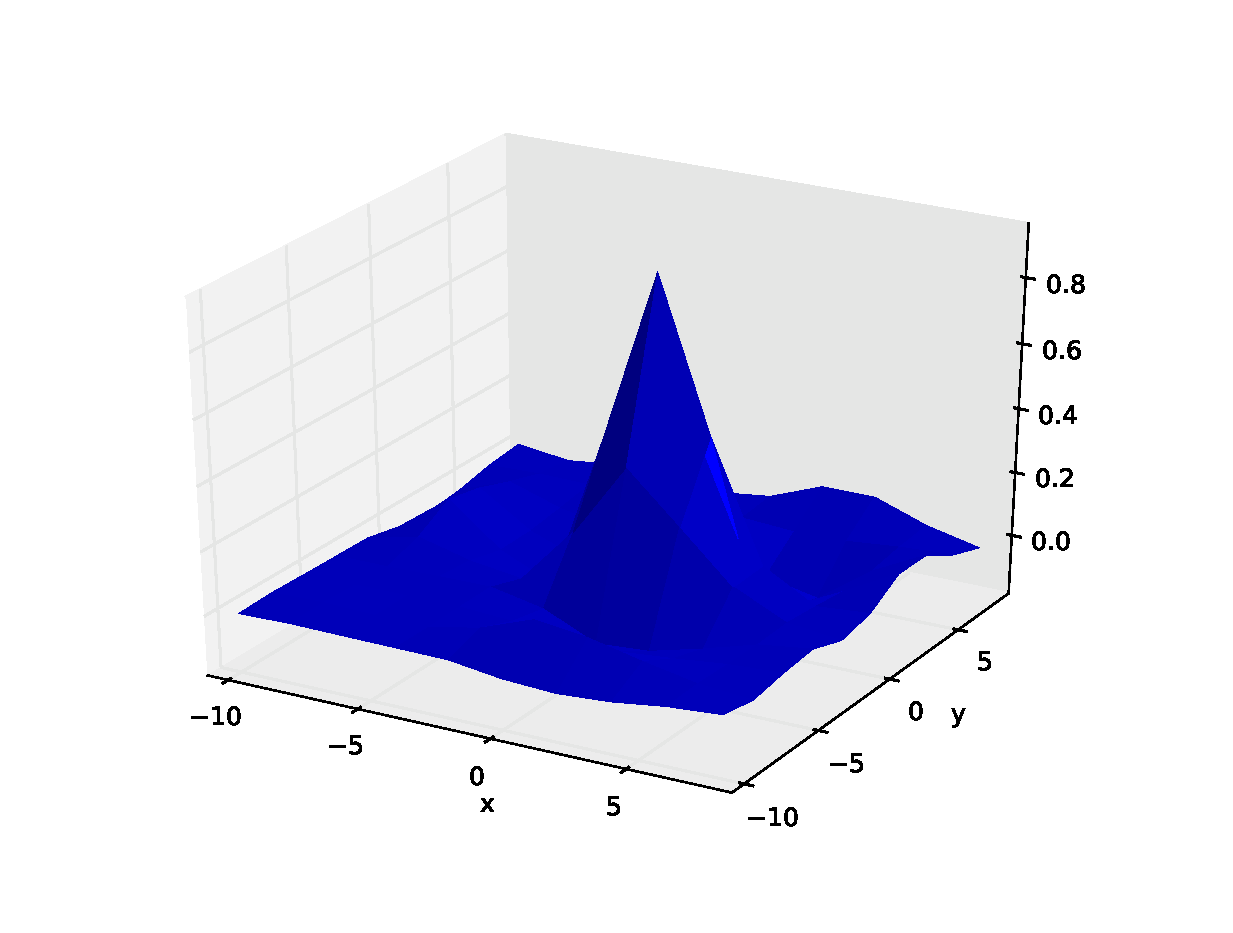
\includegraphics[width = 6cm]{train.eps}}
        \Rput[c](8,2){\small 50 epok uczenia}
\end{pspicture}
}
\section{Algorytmy ewolucyjne w strojeniu modeli rozmytych}
\frame{
\frametitle{Algorytmy ewolucyjne}
\begin{itemize}
\item Ewolucja sztucznych osobników należących do populacji
\item Rozmnażanie - Mutacja i krzyżowanie
\item Dobór naturalny
\end{itemize}
}
\subsection{Podejście oparte na dyskretyzacji}
\frame{
  \frametitle{Podejście oparte na dyskretyzacji}
  \begin{itemize}
    \item Dyskretyzacja przestrzeni zmiennych wejściowych
    \resizebox{\textwidth}{!}{
      \begin{pspicture}(10,3)
          %\psgrid
          \psaxes[labels=none, ticks=x]{->}(0,1)(0,1)(9,3)
          \psline{-}(0.5,2.5)(2.5,1)
          \psline{-}(0.5,1)(2.5,2.5)(3.5,1)
          \psline{-}(2.5,1)(3.5,2.5)(4.5,1)
          \psline{-}(3.5,1)(4.5,2.5)(7.5,1)
          \psline{-}(4.5,1)(7.5,2.5)(8.5,1)
          \psline{-}(7.5,1)(8.5,2.5)
          \Rput[rt](9,1){$x$}
          \Rput[rt](0,3){$\mu (x)$}
          \psline{-}(0,0)(9,0)
          \psline{-}(0,0.5)(9,0.5)
          \psline{-}(0,0)(0,0.5)
          \Rput[c](0.5,0.25){$1$}
          \psline{-}(1,0)(1,0.5)
          \Rput[c](1.5,0.25){$0$}
          \psline{-}(2,0)(2,0.5)
          \Rput[c](2.5,0.25){$1$}
          \psline{-}(3,0)(3,0.5)
          \Rput[c](3.5,0.25){$1$}
          \psline{-}(4,0)(4,0.5)
          \Rput[c](4.5,0.25){$1$}
          \psline{-}(5,0)(5,0.5)
          \Rput[c](5.5,0.25){$0$}
          \psline{-}(6,0)(6,0.5)
          \Rput[c](6.5,0.25){$0$}
          \psline{-}(7,0)(7,0.5)
          \Rput[c](7.5,0.25){$1$}
          \psline{-}(8,0)(8,0.5)
          \Rput[c](8.5,0.25){$1$}
          \psline{-}(9,0)(9,0.5)
          \psline[linestyle=dashed]{->}(0.5,2.5)(0.5,0.5)
          \psline[linestyle=dashed]{->}(2.5,2.5)(2.5,0.5)
          \psline[linestyle=dashed]{->}(3.5,2.5)(3.5,0.5)
          \psline[linestyle=dashed]{->}(4.5,2.5)(4.5,0.5)
          \psline[linestyle=dashed]{->}(7.5,2.5)(7.5,0.5)
          \psline[linestyle=dashed]{->}(8.5,2.5)(8.5,0.5)

      \end{pspicture}
    }

    \item Mutacja -- zamiana dwóch różnych bitów
    \item Krzyżowanie -- wymiana parzystej liczby różnych bitów
    \item Funkcja dopasowania -- suma kwadratów uchybów dla danych ze zbioru uczącego
  \end{itemize}
}
\subsection{Podejście z genotypem ciągłym}
\frame{
  \frametitle{Podejście z genotypem ciągłym}
  \begin{itemize}
    \item Genotyp -- wektor rzeczywistych parametrów modelu
    \item Mutacja -- mutacja nierównomierna
  \end{itemize}
        \begin{displaymath}
            \begin{array}{c}
                c^{l+1} = \left\{ \begin{array}{l} c^{l} + \Delta (l, \delta _{c_{\mathrm{max}}}),\quad b = 0 \\
                                                    c^{l} - \Delta (l, \delta _{c_{\mathrm{max}}}),\quad b = 1
                            \end{array} \right. \\
            \Delta (l,y) = y(1-r^{(1-\frac{l}{l_{\mathrm{max}}})^b})
            \end{array}
        \end{displaymath}
  \begin{itemize}
    \item Krzyżowanie
        \begin{displaymath}
            \begin{array}{ll}
            C_1^{l+1} = aC_r^l + (1-a)C_s^l,& C_2^{l+1} = (1-a)C_r^l + aC_s^l,\\
            C_3^{l+1} = \mathrm{min}(C_r^l, C_s^l),& C_4^{l+1} = \mathrm{max}(C_r^l, C_s^l)
            \end{array}
        \end{displaymath}
  \end{itemize}
}

\subsection*{}
\frame{
\frametitle{Inne zastosowania algorytmów ewolucyjnych}
\begin{itemize}
\item Dostrajanie parametrów liniowych następników -- reprezentacja kątowa
\item Ewolucyjny dobór struktury sieci
\item Wybór istotnych wejść modelu
\end{itemize}
}

\section{Implementacja}
\frame{
  \frametitle{Implementacja}
  \begin{itemize}
    \item Wygodne i uniwersalne API do tworzenia i strojenia modeli rozmytych
    \item Elastyczność - swoboda wyboru struktury i parametrów dostrajalnych modelu
    \item Interfejs graficzny oparty o przeglądarkę
    \item Możliwość importu i eksportu danych wykorzystywanych przez MATLAB Fuzzy Toolbox
    \item Wykorzystywane technologie: Python, NumPy, SciPy, Django
  \end{itemize}
}

\frame{
\begin{center}
  \Large
  Dziękuję za uwagę
\end{center}
}
\end{document}

